% Soundness chain laid out as a serpentine: top row reads left-to-right
% (.tree -> AST -> IR), a short vertical wrap arrow lands on SMV (under
% IR), and the bottom row reads right-to-left (SMV -> nuXmv -> T |= phi).
\documentclass[border=6pt,tikz]{standalone}
\usepackage{tikz}
\usepackage{amsmath, amssymb}
\usepackage[T1]{fontenc}
\usepackage{lmodern}
\usetikzlibrary{arrows.meta, positioning, fit, calc, backgrounds}

\tikzset{
  source/.style = {draw, rounded corners=2pt, fill=blue!10,
                   align=center, font=\scriptsize,
                   inner sep=4pt, minimum width=1.7cm, minimum height=0.9cm},
  stage/.style  = {draw, rounded corners=2pt, fill=purple!12,
                   align=center, font=\scriptsize,
                   inner sep=4pt, minimum width=1.7cm, minimum height=0.9cm},
  smv/.style    = {draw, rounded corners=2pt, fill=orange!16,
                   align=center, font=\scriptsize,
                   inner sep=4pt, minimum width=1.9cm, minimum height=0.9cm},
  decide/.style = {draw, rounded corners=2pt, fill=red!12,
                   align=center, font=\scriptsize,
                   inner sep=4pt, minimum width=1.9cm, minimum height=0.9cm},
  result/.style = {draw, rounded corners=2pt, fill=green!16, double,
                   align=center, font=\scriptsize\bfseries,
                   inner sep=4pt, minimum width=1.9cm, minimum height=0.9cm},
  flow/.style     = {-{Latex[length=2.2mm]}, line width=0.55pt,
                     shorten >=1pt, shorten <=1pt},
  edgelabel/.style= {font=\tiny, text=black!75, align=center,
                     fill=white, inner sep=1pt, rounded corners=1pt},
  claimtag/.style = {font=\tiny\bfseries, text=purple!70!black,
                     fill=white, inner sep=1pt, rounded corners=1pt},
  brace/.style    = {decorate, decoration={brace, amplitude=4pt, mirror},
                     thick, black!55},
  undernote/.style= {font=\scriptsize, text=black!75, align=center},
}

\begin{document}
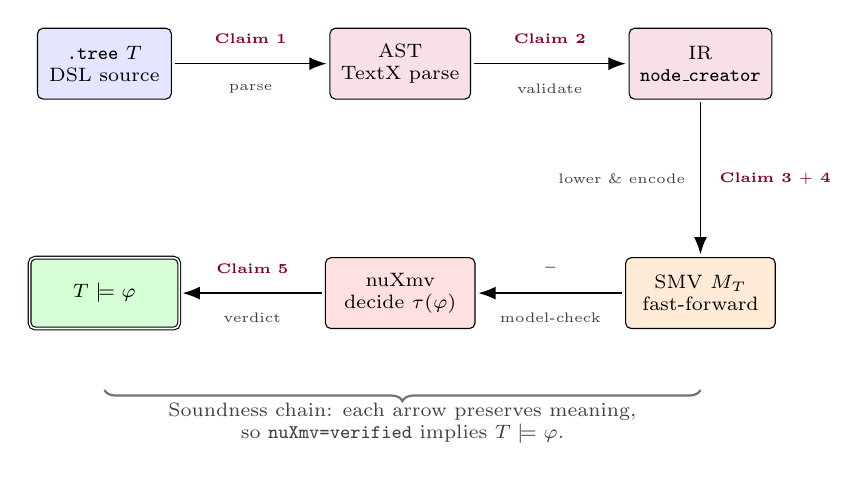
\begin{tikzpicture}[node distance=1.9cm and 2.0cm]

% ================ ROW 1 (left -> right) ================
\node[source]                 (t)   {\texttt{.tree} $T$\\\scriptsize DSL source};
\node[stage, right=of t]      (ast) {AST\\\scriptsize TextX parse};
\node[stage, right=of ast]    (ir)  {IR\\\scriptsize \texttt{node\_creator}};

\draw[flow] (t) -- (ast)
  node[midway, claimtag, yshift=9pt] {Claim 1}
  node[midway, edgelabel, yshift=-9pt] {parse};
\draw[flow] (ast) -- (ir)
  node[midway, claimtag, yshift=9pt] {Claim 2}
  node[midway, edgelabel, yshift=-9pt] {validate};

% ================ ROW 2 (right -> left) ================
% SMV sits directly below IR so the wrap arrow is a straight vertical line.
% Arrows on row 2 point right-to-left.
\node[smv,    below=2.0cm of ir]  (mt) {SMV $M_T$\\\scriptsize fast-forward};
\node[decide, below=2.0cm of ast] (nx) {nuXmv\\\scriptsize decide $\tau(\varphi)$};
\node[result, below=2.0cm of t]   (ok) {$T \models \varphi$};

\draw[flow] (mt) -- (nx)
  node[midway, claimtag, yshift=9pt] {--}
  node[midway, edgelabel, yshift=-9pt] {model-check};
\draw[flow] (nx) -- (ok)
  node[midway, claimtag, yshift=9pt] {Claim 5}
  node[midway, edgelabel, yshift=-9pt] {verdict};

% ================ WRAP: IR (end of row 1) -> SMV (start of row 2) ================
% Straight vertical arrow, labels offset to the side of the line.
\draw[flow] (ir.south) -- (mt.north);
\node[claimtag]  at ($(ir.south)!0.5!(mt.north) + (0.95cm, 0)$) {Claim 3 $+$ 4};
\node[edgelabel] at ($(ir.south)!0.5!(mt.north) + (-1.0cm, 0)$) {lower \& encode};

% ================ Bottom brace ================
\draw[brace]
      ([yshift=-22pt]ok.south) -- ([yshift=-22pt]mt.south);
\node[undernote]
      at ($(ok.south)!0.5!(mt.south) + (0,-1.2cm)$)
      {Soundness chain: each arrow preserves meaning,\\
       so \texttt{nuXmv=verified} implies $T \models \varphi$.};

\end{tikzpicture}
\end{document}
